\subsection{Continuous Integration}

The continuous integration is done with Cirrus CI. It is a free service for open-source projects that allows you to run tests on different
platforms. It is configured with a .cirrus.yml file at the root of the project. It works mostly like the local Makefile I've made to run 
the tests locally, but it uses the fact that failing test output a message with "FAIL" inside of them to detect if it should indicate that 
the running tests have failed or not. It also uses the fact that the testbench generates a .vcd file to upload it as an artifact of the build
so that you can download it and see the different signals of the simulation which can be helpful to debug the different issues.

\begin{figure}[H]
    \centering
    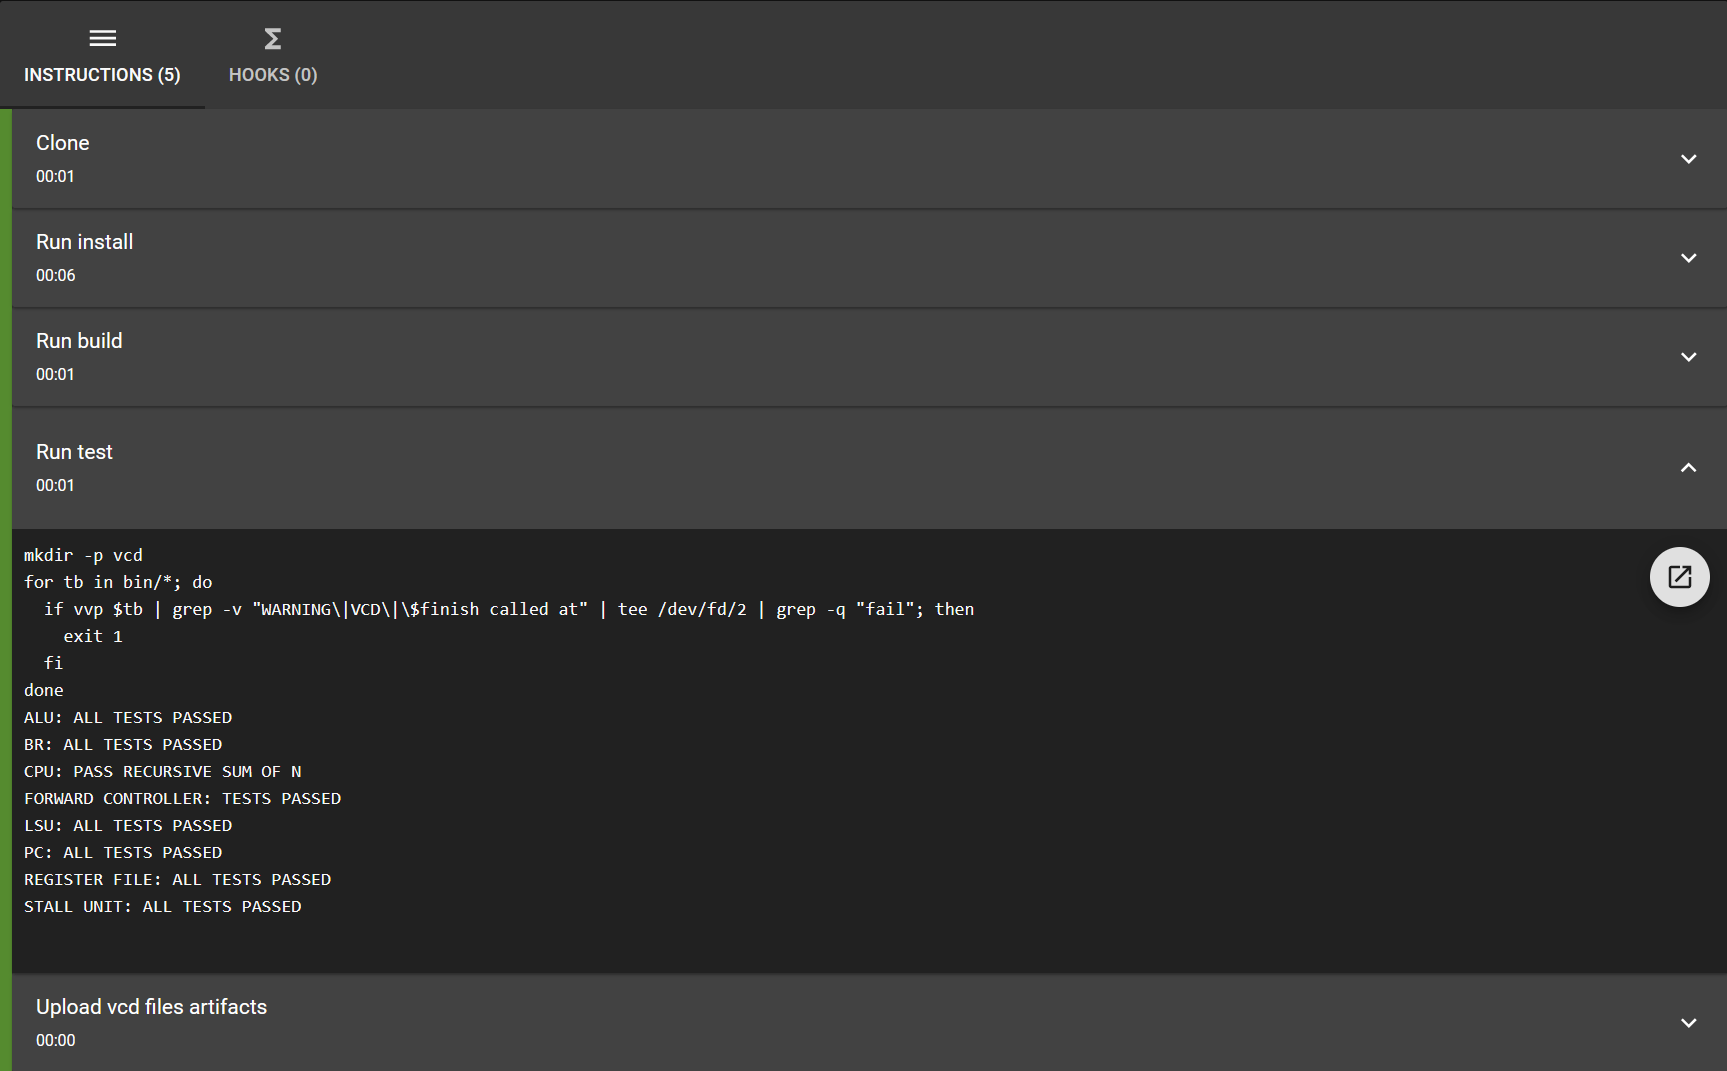
\includegraphics[width=1\textwidth]{testing/images/ci.png}
    \caption{Cirrus CI output after a commit}
    \label{fig:ci}
\end{figure}

The configuration was quite simple but I had issues after 2 weeks of using it where the docker image I was using wasn't working anymore for 
no apparent reason. So I've decided to simply use an Ubuntu environment and install the different dependencies manually. It's not a big 
deal since I've not a lot of dependencies and it's not taking a lot of time to install them. But it's still a bit annoying to have to
to pull the dependencies for each build instead of simply caching the build docker image. But it's still working fine and I'm happy with it.